% !TEX root = XRayMicroTomography.Presentation.tex

\title{X-ray microtomography}
\author{David Haberthür}
\date{December 22, 2023 | \href{https://ilias.unibe.ch/goto_ilias3_unibe_sess_2774509.html}{9256-HS2023-0: Advanced Microscopy}}

\usetheme{UniBern}

%\includeonlyframes{current}
%then....
%\begin{frame}[label=current]
%\end{frame}

% Some often used abbreviations/commands
\newcommand{\everyframe}{1}% use only every nth frame for the animations
\newcommand{\imwidth}{\linewidth}% set global image width
\newcommand{\imheight}{0.618\paperheight}% set global image height
\newlength\imagewidth% needed for scalebars
\newlength\imagescale% needed for scalebars
\newcommand{\uct}{{\textmu}CT\xspace}% make our life easier
\newcommand{\eg}{e.\,g.\xspace}%
\newcommand{\ie}{i.\,e.\xspace}%

\usepackage[backend=biber,
	style=numeric,
	url=false,
	isbn=true,
	maxnames=1,
	sorting=none]{biblatex}
\addbibresource{../../../Documents/library.bib}% FastSSD, Windows or Mac works (on Linux/FastSSD we generated a 'Document' folder at the correct level and `ln -s ~/P/Documents/library.bib .` to it)
\usepackage{standalone}
\usepackage{tikz}
	\usetikzlibrary{spy}
	\tikzset{shadowed/.style={preaction={transform canvas={shift={(1pt,-1pt)}},draw=ubRed}}}
\usepackage{shadowtext}% for the shadowed scalebar
	\shadowoffset{1pt}
	\shadowcolor{ubRed}
\usepackage{pgfplots}
	\pgfplotsset{compat=newest}
\usepackage[detect-all=true,
	range-phrase=--,
	range-units=single,
	binary-units=true,
	per-mode=symbol,
	per-symbol=/]{siunitx}
\usepackage{microtype}
\usepackage[absolute,overlay]{textpos}%for the \source{} command
\usepackage[missing=main]{gitinfo2}% GitHub Actions don't pull in the commit hash, so we just show `main'
\usepackage{xspace}
\usepackage{ccicons}
\usepackage[version=4]{mhchem}
\usepackage{animate}
\usepackage{fontawesome5}
\usepackage{csquotes}
\usepackage{listings}
	\lstset{frame=single,
		%backgroundcolor = \color{lightgray},
		basicstyle=\tiny\ttfamily
		}
\usepackage{pgfplotstable}
\usepackage{booktabs}
\usepackage{colortbl}
\usepackage{multirow}
\usepackage{lipsum}%for alignment testing
\usepackage{mathastext}

% Define complementary colors to ubRed
\definecolor{ubRedComplementary1}{HTML}{00a1e6}
\definecolor{ubRedComplementary2}{HTML}{00e645}

% change tikz font to slide font
% https://tex.stackexchange.com/a/33329/828
\usepackage[eulergreek]{sansmath}
	\pgfplotsset{tick label style = {font=\sansmath\sffamily},
		every axis label = {font=\sansmath\sffamily},
		legend style = {font=\sansmath\sffamily},
		label style = {font=\sansmath\sffamily}
		}

% Globally thicker lines in with tikz
% https://tex.stackexchange.com/a/206769/828
\tikzset{every picture/.style={thick}}

% Acknowledge images just below them
% Based on https://tex.stackexchange.com/a/282637/828
\newcommand{\source}[2]{%
	% Print out (short) link under image, with small text
	\raisebox{-1.618ex}{%
		\makebox[0pt][r]{%
			\tiny\href{http://#1}{#1} #2%
			}%
		}%
	}%
\newcommand{\sourcecite}[2]{%
	% Cite (an image from) a reference
	\raisebox{-1.618ex}{%
		\makebox[0pt][r]{%
			\tiny From \cite{#1}, #2%
			}%
		}%
	}%
\newcommand{\sourcelink}[3]{%
	% Make the source command an \href{link}{text}
	\raisebox{-1.618ex}{%
		\makebox[0pt][r]{%
			\tiny\href{http://#1}{#2}, #3%
			}%
		}%
	}%

% Define us a custom footer *with* progress bar, based on https://tex.stackexchange.com/a/59749/828
\makeatletter
\def\progressbar@progressbar{}% the progress bar
\newcount\progressbar@tmpcounta% auxiliary counter
\newcount\progressbar@tmpcountb% auxiliary counter
\newdimen\progressbar@pbht%progressbar height
\newdimen\progressbar@pbwd%progressbar width
\newdimen\progressbar@rcircle% radius for the circle
\newdimen\progressbar@tmpdim% auxiliary dimension
\progressbar@pbwd=0.85\linewidth%
\progressbar@rcircle=1.5pt%
\def\progressbar@progressbar{%
	\progressbar@tmpcounta=\insertframenumber%
	\progressbar@tmpcountb=\inserttotalframenumber%
	\progressbar@tmpdim=\progressbar@pbwd%
	\multiply\progressbar@tmpdim by \progressbar@tmpcounta%
	\divide\progressbar@tmpdim by \progressbar@tmpcountb%
	\par%
		\mode<beamer>{%
			\begin{tikzpicture}%
				\draw[ubGrey] (0,0) -- ++ (\progressbar@pbwd,0);%
				\draw[draw=ubRed,fill=ubGrey] (\the\dimexpr\progressbar@tmpdim-\progressbar@rcircle\relax,.5\progressbar@pbht) circle (\progressbar@rcircle);%
			\end{tikzpicture}%
			\hfill git.io/JqIBH\xspace|\xspace%
			v. \href{https://github.com/habi/Lecture.Microtomography/commit/\gitHash}{\gitAbbrevHash}\xspace|\xspace%
			p.\xspace\insertframenumber/\inserttotalframenumber%
			}%
		\mode<handout>{%
			git.io/JqIBH\hfill|\hfill%
			Handout created on \DTMnow\hfill|\hfill%
			p.\xspace\insertframenumber/\inserttotalframenumber%
			}%
		\vspace{0.5ex}%
}

\addtobeamertemplate{footline}{}%
{%
	\begin{beamercolorbox}[wd=\paperwidth,center]{green}%
		\progressbar@progressbar%
	\end{beamercolorbox}%
}%
\makeatother

% Format bibliography for beamer
% http://tex.stackexchange.com/a/10686/828
\renewbibmacro{in:}{}
% http://tex.stackexchange.com/a/13076/828
\AtEveryBibitem{%
	\clearfield{journaltitle}
	\clearfield{pages}
	\clearfield{volume}
	\clearfield{number}
	\clearname{editor}
	\clearfield{issn}
	\clearfield{year}
}
% No parentheses around the (now empty) year: https://tex.stackexchange.com/a/147537/828
\renewcommand{\bibopenparen}{\addcomma\addspace}
\renewcommand{\bibcloseparen}{\addcomma\addspace}

% Redefine \footcite based on https://tex.stackexchange.com/a/453528/828
\DeclareCiteCommand{\footcite}[\mkbibfootnote]{%
	\usebibmacro{prenote}}{%
		\printnames[family-given]{labelname}%
		\newunit%
		\printfield{doi}%
		\newunit%
		\printlabeldateextra%
	}{\addsemicolon\space}{%
		\usebibmacro{postnote}%
	}%

% References as footnotes at the bottom of the slides
% https://tex.stackexchange.com/a/368760/828
\makeatletter
\renewcommand\@makefnmark{\xspace\hbox{\usebeamercolor[fg]{footnote mark}\usebeamerfont*{footnote mark}[\@thefnmark]}}
\renewcommand\@makefntext[1]{\tiny{\usebeamercolor[fg]{footnote mark}\usebeamerfont*{footnote mark}[\@thefnmark]}\enspace\usebeamerfont*{footnote} #1}
\makeatother

% Show current section at begin of sections, but only in presentation mode
\mode<beamer>{%
	\AtBeginSection[]{%
		\begin{frame}{Contents}
			\tableofcontents[currentsection,currentsubsection,hideothersubsections]
		\end{frame}
	}
}

% Slide transiton
%\addtobeamertemplate{background canvas}{\transfade[duration=0.5]}{}

% open in fullscreen
%\hypersetup{pdfpagemode=FullScreen}

% Move the text down a bit
% THIS IS A BIG HACK, IT SHOULD BE FIXED IN THE TEMPLATE
\addtobeamertemplate{frametitle}{}{\vspace*{0.75em}}

\begin{document}
% No footline on the title page
% http://tex.stackexchange.com/a/18829/828 helps us to achieve that
{%
	\setbeamertemplate{footline}{}%
	\begin{frame}%
		\maketitle
	\end{frame}%
}

%% Alignment frames to test the ugly text-block-movement hack above
%\begin{frame}[label=current]{Alignment frame}
%	\begin{tikzpicture}%
%		\def\cut{2}%
%		\draw [|-|,ultra thick] (0,\cut) -- (0,\textheight-\cut);%
%		\draw [<->,ultra thick] (0.5\textwidth,\cut) -- (0.5\textwidth,\textheight-\cut);%
%		\draw [|-|,ultra thick] (\textwidth,\cut) -- (\textwidth,\textheight-\cut);%
%	\end{tikzpicture}%
%\end{frame}
%
%\begin{frame}[allowframebreaks,label=current]{Alignment frame II}
%	\lipsum[1-3]
%\end{frame}

\begin{frame}
	\frametitle{Grüessech!}
	\begin{itemize}
		\item David Haberthür
		\begin{itemize}
			\item Physicist by trade
			\item \href{https://boris.unibe.ch/2619/}{PhD in high resolution imaging of the lung}, Institute of Anatomy, University of Bern, Switzerland
			\item Post-Doc I: Tomographic imaging at \href{https://www.psi.ch/sls/tomcat/}{TOMCAT}, \href{https://www.psi.ch/sls/}{Swiss Light Source}, \href{https://www.psi.ch/}{Paul Scherrer Institute}, Switzerland and working on the detector of the \href{http://globaldiagnostix.org}{GlobalDiagnostiX} project
			\item Post-Doc II \& currently: Tomographic imaging in the \href{https://www.ana.unibe.ch/forschung/mikroct/research/}{\uct group}, Institute of Anatomy, University of Bern, Switzerland
		\end{itemize}
	\end{itemize}
\end{frame}

\begin{frame}
	\frametitle{\uct-group}
	\begin{columns}
		\begin{column}{0.61\linewidth}
			\begin{itemize}
				\item microangioCT~\cite{Hlushchuk2018}
				\begin{itemize}
					\item Angiogenesis: heart, musculature~\cite{Nording2021} and bones
					\item Vasculature: (mouse) brain~\cite{Hlushchuk2020}, (human) nerve scaffolds~\cite{Wuthrich2020}, (human) skin flaps~\cite{Zubler2021} and tumors
				\end{itemize}
				\item Zebrafish musculature and gills~\cite{MesserliAaldijk2020}
				\item (Lung) tumor detection and metastasis classification~\cite{Trappetti2021}
				\item Collaborations with museums~\cite{Bochud2021} and scientist at UniBe~\cite{Halm2021} to scan a wide range of specimens
				\item Automate \emph{all} the things!~\cite{Haberthur2021}
			\end{itemize}
		\end{column}
		\begin{column}{0.37\linewidth}
			\centering
			\includegraphics<1|handout:0>[width=\imwidth]{./images/1172}%
			\only<1|handout:0>{\source{brukersupport.com}{}}
			\includegraphics<2>[width=\imwidth]{./images/1272}%
			\only<2>{\source{bruker.com/skyscan1272}{}}
			\includegraphics<3|handout:0>[width=\imwidth]{./images/2214}%
			\only<3|handout:0>{\source{bruker.com/skyscan2214}{}}
		\end{column}
	\end{columns}
\end{frame}

\begin{frame}{Contents}
	\tableofcontents
\end{frame}

\section{Overview}
\begin{frame}
	\frametitle{Biomedical imaging}%
	\begin{columns}%
		\begin{column}{0.37\linewidth}%
			\begin{itemize}%
				\item<1-|handout:1-> Medical research%
				\item<1-|handout:1-> Non-destructive insights into the samples%
				\item<2-|handout:1->(Small) biological samples%
			\end{itemize}%
		\end{column}%
		\begin{column}{0.61\linewidth}%
			\centering%
			\only<1-2|handout:1>{%
				\includegraphics[height=\imheight]{./images/Sagittal_brain_MRI}%
				\source{w.wiki/7g4}{\ccbysa}%
			}%
			\only<3|handout:2>{%
				\begin{tikzpicture}[remember picture,overlay]%
					\node at (current page.center){%
						\mode<beamer>{\animategraphics[loop,autoplay,width=\paperwidth,every=\everyframe]{24}{./movies/mouse_skull/mouse_skull}{000}{236}}%
						\mode<handout>{\includegraphics[width=\paperwidth]{./movies/mouse_skull/mouse_skull075}}
					};%
				\end{tikzpicture}%
			}%
		\end{column}%
	\end{columns}%
\end{frame}

\section{Imaging}
\begin{frame}
	\frametitle{Wavelength and scales}
	\centering
	\only<1|handout:1>{%
		\includegraphics[height=\imheight]{./images/2000px-Electromagnetic_spectrum_with_sources}%
		\source{w.wiki/7fz}{\ccbysa}%
		}%
	\only<2|handout:2>{%
		\includegraphics[height=\imheight]{./images/MIC-AM_techniques}%
		\sourcelink{https://anatomie.unibe.ch/tschanz}{Stefan Tschanz}{with permission}%
		}
\end{frame}

\begin{frame}
	\frametitle{Imaging methods}
	\begin{itemize}
		\item Light (sheet) microscopy: see \href{https://ilias.unibe.ch/goto_ilias3_unibe_sess_2774495.html}{lecture of Myra Chavez}
		\item X-ray imaging
		\item Electron microscopy: see lectures
			\href{https://ilias.unibe.ch/goto_ilias3_unibe_sess_2774501.html}{\emph{Transmission Electron Microscopy} by Dimitri Vanhecke},
			\href{https://ilias.unibe.ch/goto_ilias3_unibe_sess_2774505.html}{\emph{Scanning Electron Microscopy} by Sabine Kässmeyer \& Ivana Jaric} and
			\href{https://ilias.unibe.ch/goto_ilias3_unibe_sess_2774507.html}{\emph{Cryoelectron Microscopy \& Serial Block Face SEM} by Ioan Iacovache}.
	\end{itemize}
\end{frame}

\section{Tomography}
\begin{frame}
	\frametitle{CT-Scanner}
	\centering
	\mode<beamer>{%
		\animategraphics[loop,height=\imheight,every=\everyframe]{24}{./movies/ct-scanner/ct-scanner0}{001}{480}%
		\source{youtu.be/2CWpZKuy-NE}{}%
		}
	\mode<handout>{%
		\includegraphics[height=\imheight]{./movies/ct-scanner/ct-scanner0001}%
		\source{youtu.be/2CWpZKuy-NE}{}%
		}
\end{frame}
\note{From \href{https://www.bruker.com/products/microtomography/micro-ct-for-sample-scanning/x-ray-micro-ct-microtomography.html}{Bruker Homepage}:
	Micro computed tomography or micro-CT is X-ray imaging in 3D, by the same method used in hospital CT (or CAT) scans, but on a small scale with massively increased resolution.
	It represents proper "3D microscopy", where very fine scale internal structure of objects is imaged non-destructively.
	No sample preparation, no staining, no thin slicing---a single scan will image your sample's complete internal 3D structure at high resolution, plus you get your intact sample back at the end!}

\subsection{History}
\renewcommand{\imwidth}{\columnwidth}
\begin{frame}
	\frametitle{History}
	\begin{columns}
		\begin{column}{0.49\linewidth}
			\begin{itemize}
				\item Long history
				\begin{itemize}
					\item \citeyear{Cormack1963}:~\citeauthor{Cormack1963} used a collimated \ce{^{60}Co} source and a Geiger counter as a detector~\cite{Cormack1963}%
					\item 1976:~\citeauthor{Hounsfield1976a} worked on first clinical scanner~\cite{Hounsfield1976a}%
					\item Nice overview by \citeauthor{Hsieh2003}~\cite{Hsieh2003}%
				\end{itemize}%
				\item<2-|handout:2-> CT scanner generations: First\uncover<3-|handout:3->{, second}\uncover<4|handout:4->{ and third}%
			\end{itemize}
		\end{column}
		\begin{column}{0.49\linewidth}
			\centering
			\only<1|handout:1>{%
				\renewcommand{\imwidth}{0.714769648*\imheight}% 1055/1476
				\pgfmathsetlength{\imagewidth}{\imwidth}%
				\pgfmathsetlength{\imagescale}{\imagewidth/1055}%
				\def\x{652}% scalebar-x starting at golden ratio of image width of 1055px = 652
				\def\y{1328}% scalebar-y at 90% of image height of 1476px = 1328
				\begin{tikzpicture}[x=\imagescale,y=-\imagescale]
					\node[anchor=north west, inner sep=0pt, outer sep=0pt] at (0,0) {\includegraphics[width=\imagewidth]{./images/first_ct_image}};
					% 633.730px = 160.00000004mm -> 100px = 25247.344um -> 1.980px = 500um, 0.396px = 100um
					%\draw[|-|,blue,thick] (224,832) -- (858,826) node [sloped,midway,above,fill=white,semitransparent,text opacity=1] {\SI{160.00000004}{\milli\meter} (634px) TEMPORARY!};
					\draw[|-|,white,thick,shadowed] (\x,\y) -- (\x+198.0,\y) node [midway,above] {\shadowtext{\SI{5}{\centi\meter}}};
				\end{tikzpicture}%
			}%
			\only<1|handout:1>{\sourcecite{Beckmann2006}{Figure 5}}%
			\includegraphics<2|handout:2>[width=\imwidth]{./images/History_Generation1}%
			\only<2|handout:2>{\sourcecite{Hsieh2003}{Figure 1.12}}%
			\includegraphics<3|handout:3>[width=\imwidth]{./images/History_Generation2}%
			\only<3|handout:3>{\sourcecite{Hsieh2003}{Figure 1.13}}%
			\includegraphics<4|handout:4>[width=\imwidth]{./images/History_Generation3}%
			\only<4|handout:4>{\sourcecite{Hsieh2003}{Figure 1.14}}%
		\end{column}
	\end{columns}
\end{frame}
\note{We were unable to find any information on the voxel size of the first CT image.
	My head is approximately 16 cm wide.
	I counted 47 voxels across the head in the image.
	This gives a voxel size of 3.4 mm per voxel.
}

\subsection{Interaction of X-rays with matter}
\begin{frame}
	\frametitle{X-ray interaction}
	\begin{itemize}
		\item \textquote[\cite{xrayphysics}]{X-rays interact with tissue in 2 main ways: photoelectric effect and Compton scatter.
				To a first approximation, the photoelectric effect contributes to contrast while the Compton effect contributes to noise.
				Both contribute to dose.}
		\begin{itemize}
			\item Photoelectric absorption (\(\tau\)) is strongly dependent on the atomic number \(Z\) of the absorbing material: \(\tau\propto\frac{Z^4}{E^{3.5}}\)
			\item Compton scattering is one of the principle forms of photon interaction and is directly proportional to the electron density and physical density of the material.
				Compton scattering does \emph{not} depend on the atomic number: \(\lambda'-\lambda=\frac{h}{m_{e}c}\left(1-\cos{\theta}\right)\)
		\end{itemize}
		\item Lowering X-ray energy increases contrast
		\item X-ray penetration decreases exponentially with sample thickness (\cite[\ie Beer-Lamberts law]{wiki:beer-lambert} \(I(t)=I_{0}e^{-\alpha z}\)
	\end{itemize}
\end{frame}
\note{From \href{https://radiopaedia.org/articles/photoelectric-effect}{radiopaedia.org}: Therefore if \(Z\) doubles, PEA will increase by a factor of 16 (\(2^4=16\)), and if \(E\) doubles PEA will be reduced by a factor of 11.
    Small changes in \(Z\) and \(E\) can therefore significantly affect PEA.
	This has practical implications in the field of radiation protection and is the reason materials with a high \(Z\) such as lead (\(Z= 82\)) are useful shielding materials.
	The dependence of PEA on \(Z\) and \(E\) means that it is the major contributor to beam attenuation up to approximately \SI{30}{\kilo\electronvolt} when human tissues (\(Z=7.4\)) are irradiated.
	At beam energies above this, the Compton effect predominates.}
\note{Where \(\lambda\) is the initial wavelength, \(\lambda'\) is the wavelength after scattering, \(h\) is the Planck constant, \(m_{e}\) is the electron rest mass, \(c\) is the speed of light, and \(\theta\) is the scattering angle.}

\begin{frame}
	\frametitle{Composition of biological tissues}
	Tissue: content by mass percentage
	\centering
	\begin{table}%
		\only<1>{%
			\pgfplotstabletypeset[%
				col sep=comma,% the seperator in our .csv file
				display columns/0/.style={string type},%
				% section 3.2 in pgfplotstable manual
				every head row/.style={before row={\toprule}},%
				every row no 0/.style={after row=\midrule},%
				every last row/.style={after row=\bottomrule},%
			]{./tables/tissue-composition.csv}%
		}%
		\only<2|handout:0>{%
			\pgfplotstabletypeset[%
				col sep=comma,% the seperator in our .csv file
				display columns/0/.style={string type},%
				every head row/.style={before row={\toprule}},%
				every row no 0/.style={after row=\midrule},%
				every last row/.style={after row=\bottomrule},%
				% make certain cells ubRed, based on https://tex.stackexchange.com/a/296914/828
				every row 1 column 2/.style={postproc cell content/.append style={/pgfplots/table/@cell content/.add={\cellcolor{ubRed!61.8}}{}}},%
				every row 1 column 4/.style={postproc cell content/.append style={/pgfplots/table/@cell content/.add={\cellcolor{ubRed!61.8}}{}}},%
				every row 2 column 4/.style={postproc cell content/.append style={/pgfplots/table/@cell content/.add={\cellcolor{ubRed!61.8}}{}}},%
				every row 6 column 4/.style={postproc cell content/.append style={/pgfplots/table/@cell content/.add={\cellcolor{ubRed!61.8}}{}}},%
				every row 6 column 6/.style={postproc cell content/.append style={/pgfplots/table/@cell content/.add={\cellcolor{ubRed!61.8}}{}}},%
				every row 6 column 10/.style={postproc cell content/.append style={/pgfplots/table/@cell content/.add={\cellcolor{ubRed!61.8}}{}}}%
			]{./tables/tissue-composition.csv}%
		}%
	\end{table}
\end{frame}
\note{Bone, lean tissue, fat and air can be distinguished easily}

\begin{frame}
	\frametitle{Why \uct?}
	\begin{columns}
		\begin{column}{0.49\linewidth}
			% https://www.cancerimagingarchive.net/nbia-search/?saved-cart=nbia-76761575299081509
			\only<1-4|handout:1-4>{%
				\pgfmathsetlength{\imagewidth}{\imwidth}%
				\pgfmathsetlength{\imagescale}{\imagewidth/512}%
				\def\x{316}% scalebar-x starting at golden ratio of image width of 512px = 316
				\def\y{361}% scalebar-y at 90% of image height of 401px = 361
				\begin{tikzpicture}[x=\imagescale,y=-\imagescale]
					\node[anchor=north west, inner sep=0pt, outer sep=0pt] at (0,0) {\includegraphics[width=\imagewidth]{./images/comparison/MAX_human}};
					% 512.000px = 250.0096mm -> 100px = 48830.000um -> 1.024px = 500um, 0.205px = 100um
					%\draw[|-|,blue,thick] (0,200) -- (512,200) node [sloped,midway,above,fill=white,semitransparent,text opacity=1] {\SI{250.0096}{\milli\meter} (512px) TEMPORARY!};
					\draw[|-|,white,shadowed] (\x,\y) -- (\x+102.4,\y) node [midway,above] {\shadowtext{\SI{5}{\centi\meter}}};
				\end{tikzpicture}%
			}%
			\only<5|handout:0>{%
				\pgfmathsetlength{\imagewidth}{\imwidth}%
				\pgfmathsetlength{\imagescale}{\imagewidth/512}%
				\def\x{316}% scalebar-x starting at golden ratio of image width of 512px = 316
				\def\y{361}% scalebar-y at 90% of image height of 401px = 361
				\def\mag{6}% magnification of inset
				\def\size{125}% size of inset
				\begin{tikzpicture}[x=\imagescale,y=-\imagescale,spy using outlines={rectangle,magnification=\mag,size=\size,connect spies}]
					\node[anchor=north west, inner sep=0pt, outer sep=0pt] at (0,0) {\includegraphics[width=\imagewidth]{./images/comparison/MAX_human}};
					\spy [ubRed] on (58,356) in node at (256,201) [anchor=center];
					% 512.000px = 250.0096mm -> 100px = 48830.000um -> 1.024px = 500um, 0.205px = 100um
					\draw[|-|,white,shadowed] (\x,\y) -- (\x+102.4,\y) node [midway,above] {\shadowtext{\SI{5}{\centi\meter}}};
				\end{tikzpicture}%
			}%
			\renewcommand{\imwidth}{0.1554\columnwidth}%
			\only<6|handout:5>{%
				\centering
				\pgfmathsetlength{\imagewidth}{\imwidth}%
				\pgfmathsetlength{\imagescale}{\imagewidth/512}%
				\def\x{316}% scalebar-x starting at golden ratio of image width of 512px = 316
				\def\y{361}% scalebar-y at 90% of image height of 401px = 361
				\begin{tikzpicture}[x=\imagescale,y=-\imagescale]
					\node[anchor=north west, inner sep=0pt, outer sep=0pt] at (0,0) {\includegraphics[width=\imagewidth]{./images/comparison/MAX_human}};
					% 512.000px = 250.0096mm -> 100px = 48830.000um -> 1.024px = 500um, 0.205px = 100um
					\draw[|-|,white,shadowed] (\x,\y) -- (\x+102.4,\y) node [midway,above] {\shadowtext{\SI{5}{\centi\meter}}};
				\end{tikzpicture}%
			}%
			\sourcecite{Clark2013}{Subject \emph{C3L-02465}}
		\end{column}%
		\begin{column}{0.49\linewidth}
			\only<1|handout:1>{%
				\pgfmathsetlength{\imagewidth}{\imwidth}%
				\pgfmathsetlength{\imagescale}{\imagewidth/3295}%
				\def\x{2036}% scalebar-x starting at golden ratio of image width of 3295px = 2036
				\def\y{1343}% scalebar-y at 90% of image height of 1492px = 1343
				\begin{tikzpicture}[x=\imagescale,y=-\imagescale]
					\node[anchor=north west, inner sep=0pt, outer sep=0pt] at (0,0) {\includegraphics[width=\imagewidth]{./images/comparison/MAX_mouse}};
					% 3295.000px = 26.2282mm -> 100px = 796.000um -> 62.814px = 500um, 12.563px = 100um
					%\draw[|-|,blue,thick] (0,746) -- (3295,746) node [sloped,midway,above,fill=white,semitransparent,text opacity=1] {\SI{26.2282}{\milli\meter} (3295px) TEMPORARY!};
					\draw[|-|,white,shadowed] (\x,\y) -- (\x+628.14,\y) node [midway,above] {\shadowtext{\SI{5}{\milli\meter}}};
				\end{tikzpicture}%
			}%
			\renewcommand{\imwidth}{0.1\columnwidth}%
			\only<2|handout:2>{%
				\centering
				\pgfmathsetlength{\imagewidth}{\imwidth}%
				\pgfmathsetlength{\imagescale}{\imagewidth/54}%
				\def\x{33}% scalebar-x starting at golden ratio of image width of 54px = 33
				\def\y{22}% scalebar-y at 90% of image height of 24px = 22
				\begin{tikzpicture}[x=\imagescale,y=-\imagescale]
					\node[anchor=north west, inner sep=0pt, outer sep=0pt] at (0,0) {\includegraphics[width=\imagewidth]{./images/comparison/MAX_mouse_488umppx}};
					% 54.000px = 26.3682mm -> 100px = 48830.000um -> 1.024px = 500um, 0.205px = 100um
					%\draw[|-|,blue,thick] (0,12) -- (54,12) node [sloped,midway,above,fill=white,semitransparent,text opacity=1] {\SI{26.3682}{\milli\meter} (54px) TEMPORARY!};
					\draw[|-|,white,shadowed] (\x,\y) -- (\x+102.4,\y) node [midway,above] {\shadowtext{\SI{5}{\centi\meter}}};
					%\draw[color=red, anchor=south west] (0,24) node [fill=white, semitransparent] {Legend} node {Legend};
				\end{tikzpicture}%
			}%
			\renewcommand{\imwidth}{\columnwidth}
			\only<3|handout:3>{%
				\centering
				\pgfmathsetlength{\imagewidth}{\imwidth}%
				\pgfmathsetlength{\imagescale}{\imagewidth/54}%
				\def\x{33}% scalebar-x starting at golden ratio of image width of 54px = 33
				\def\y{22}% scalebar-y at 90% of image height of 24px = 22
				\begin{tikzpicture}[x=\imagescale,y=-\imagescale]
					\node[anchor=north west, inner sep=0pt, outer sep=0pt] at (0,0) {\includegraphics[width=\imagewidth]{./images/comparison/MAX_mouse_488umppx}};
					% 54.000px = 26.3682mm -> 100px = 48830.000um -> 1.024px = 500um, 0.205px = 100um
					%\draw[|-|,blue,thick] (0,12) -- (54,12) node [sloped,midway,above,fill=white,semitransparent,text opacity=1] {\SI{26.3682}{\milli\meter} (54px) TEMPORARY!};
					\draw[|-|,white,shadowed] (\x,\y) -- (\x+10.24,\y) node [midway,above] {\shadowtext{\SI{5}{\milli\meter}}};
					%\draw[color=red, anchor=south west] (0,24) node [fill=white, semitransparent] {Legend} node {Legend};
				\end{tikzpicture}%
			}%
			\only<4|handout:4>{%
				\pgfmathsetlength{\imagewidth}{\imwidth}%
				\pgfmathsetlength{\imagescale}{\imagewidth/3295}%
				\def\x{2036}% scalebar-x starting at golden ratio of image width of 3295px = 2036
				\def\y{1343}% scalebar-y at 90% of image height of 1492px = 1343
				\begin{tikzpicture}[x=\imagescale,y=-\imagescale]
					\node[anchor=north west, inner sep=0pt, outer sep=0pt] at (0,0) {\includegraphics[width=\imagewidth]{./images/comparison/MAX_mouse}};
					% 3295.000px = 26.2282mm -> 100px = 796.000um -> 62.814px = 500um, 12.563px = 100um
					\draw[|-|,white,shadowed] (\x,\y) -- (\x+628.14,\y) node [midway,above] {\shadowtext{\SI{5}{\milli\meter}}};
				\end{tikzpicture}%
			}%
			\only<5|handout:0>{%
				\pgfmathsetlength{\imagewidth}{\imwidth}%
				\pgfmathsetlength{\imagescale}{\imagewidth/3295}%
				\def\x{2036}% scalebar-x starting at golden ratio of image width of 3295px = 2036
				\def\y{1343}% scalebar-y at 90% of image height of 1492px = 1343
				\def\mag{6}% magnification of inset
				\def\size{125}% size of inset
				\begin{tikzpicture}[x=\imagescale,y=-\imagescale,spy using outlines={rectangle,magnification=\mag,size=\size,connect spies}]
					\node[anchor=north west, inner sep=0pt, outer sep=0pt] at (0,0) {\includegraphics[width=\imagewidth]{./images/comparison/MAX_mouse}};
					\spy [ubRed] on (352,1116) in node at (1648,746) [anchor=center];
					% 3295.000px = 26.2282mm -> 100px = 796.000um -> 62.814px = 500um, 12.563px = 100um
					\draw[|-|,white,shadowed] (\x,\y) -- (\x+628.14,\y) node [midway,above] {\shadowtext{\SI{5}{\milli\meter}}};
				\end{tikzpicture}%
			}%
			\only<6|handout:5>{%
				\pgfmathsetlength{\imagewidth}{\imwidth}%
				\pgfmathsetlength{\imagescale}{\imagewidth/3295}%
				\def\x{2036}% scalebar-x starting at golden ratio of image width of 3295px = 2036
				\def\y{1343}% scalebar-y at 90% of image height of 1492px = 1343
				\begin{tikzpicture}[x=\imagescale,y=-\imagescale]
					\node[anchor=north west, inner sep=0pt, outer sep=0pt] at (0,0) {\includegraphics[width=\imagewidth]{./images/comparison/MAX_mouse}};
					% 3295.000px = 26.2282mm -> 100px = 796.000um -> 62.814px = 500um, 12.563px = 100um
					\draw[|-|,white,shadowed] (\x,\y) -- (\x+628.14,\y) node [midway,above] {\shadowtext{\SI{5}{\milli\meter}}};
				\end{tikzpicture}%
			}%
		\end{column}
	\end{columns}
\end{frame}
\note{The human head scan was downloaded from the \href{https://www.cancerimagingarchive.net}{Cancer Imaging Archive}.
	We loaded the DICOM slices in Fiji, resliced it to show it from the side and then used to generate an MIP.
	According to the DICOM tags, the voxel size is \qtyproduct{0.4883 x 0.4883 x 0.625}{\milli\meter}, the image size is 512\(\times\)512 pixels.
	The mouse head is the same as shown in the early animation.
	The files from the early animation were resized 0.25 times; here we used the original dataset (Mouse1265\_Skull\_Gaby\_TKI\_7\_96um\_Al05\_2K) for a reslice and the generation of the MIP.
	The voxel size of the original data is 7.96 um, the image size is 3295\(\times\)1492 pixels.
}

\begin{frame}
	\frametitle{Maximum intensity projection}
	\centering
	% pdfseparate 220923_Fundamentals_image_processing_2022_Witz.pdf -f 23 -l 23 220923_Fundamentals_image_processing_2022_Witz-%d.pdf
	\includegraphics[height=\imheight]{./images/220923_Fundamentals_image_processing_2022_Witz-23}%
	\sourcelink{ilias.unibe.ch/goto_ilias3_unibe_sess_2466919.html}{\emph{Fundamentals of Digital Image Processing (2022)} by Guillaume Witz}{Slide 23}%
\end{frame}

\subsection{Tomography today}
\renewcommand{\imwidth}{\columnwidth}
\begin{frame}
	\frametitle{Machinery}
	\begin{columns}%
		\begin{column}{0.49\linewidth}%
			\begin{itemize}%
				\item<1-> Hospital CT%
				\begin{itemize}%
					\item Voxel size around \SI{0.5}{\milli\meter}%
				\end{itemize}%
				\item<2-> Lab/Desktop CT%
				\begin{itemize}%
					\item Voxel size around \SI{7}{\micro\meter} (\emph{in vivo}) or \SI{0.5}{\micro\meter} (\emph{ex vivo})%
				\end{itemize}%
				\item<4-> Synchrotron CT%
				\begin{itemize}%
					\item Voxel size down to \href{https://www.psi.ch/en/sls/tomcat/detectors}{\SI{160}{\nano\meter}}%
				\end{itemize}%
			\end{itemize}%
		\end{column}%
		\begin{column}{0.49\linewidth}%
			\centering%
			\includegraphics<1|handout:1>[width=\imwidth]{./images/24324062640_751e011e1a_o}%
			\only<1|handout:1>{\source{flic.kr/p/D4rbom}{\ccbyncsa}}%
			\includegraphics<2|handout:2>[height=\imheight]{./images/9459311320_516179207a_o}%
			\only<2|handout:2>{\source{flic.kr/p/fpTrGu}{\ccbysa}}%
			\includegraphics<3|handout:3>[width=\imwidth]{./images/1272}%
			\only<3|handout:3>{\source{bruker.com/skyscan1272}{}}%
			\includegraphics<4|handout:4>[width=\imwidth]{./images/4563733710_f632792416_b}%
			\only<4|handout:4>{\source{flic.kr/p/7Xhk2Y}{\ccbync}}%
		\end{column}%
	\end{columns}%
\end{frame}
\note{FAN BEAM -> BRUKER\newline
	PARALLEL BEAM -> TOMCAT\newline
	HELICAL/SPIRAL CT\newline
	MULTISLICE CT -> HOSPITAL
}

\begin{frame}
	\frametitle{What is happening?}
	\begin{columns}%
		\begin{column}{0.49\linewidth}%
			The basic components of a computer tomography device are always
			\begin{itemize}
				\item an X-ray source
				\item something to image
				\item a detector
			\end{itemize}
		\end{column}%
		\begin{column}{0.49\linewidth}%
			\centering%
			\includegraphics[width=\imwidth]{./images/3D_Computed_Tomography}%
			\source{w.wiki/7g3}{\ccbysa}%
		\end{column}%
	\end{columns}%
\end{frame}

\begin{frame}
	\frametitle{Machinery}
	\begin{columns}
		\begin{column}{0.49\linewidth}
			\centering
			%\documentclass{beamer}% For self-contained compilation
\documentclass[tikz]{standalone}% For inclusion in the presentation
% Draw the setup where the source and detector move, e.g. classic CT
% With help from https://tex.stackexchange.com/q/515519/828
\usepackage{animate}
\usepackage{tikz}
%	\usetikzlibrary{external}
%	\tikzexternalize
%	\tikzsetnextfilename{classicCT}
\usepackage{fontawesome5}
\usepackage{ifthen}
\ifthenelse{\isundefined{\everyframe}}{%
	% If we're compiling this file via \input, then these variables are already defined.
	% In the other case, we need to define them
	\newcommand{\everyframe}{5}
	\definecolor{ubRed}{HTML}{e4003c}%
	\definecolor{ubGrey}{HTML}{646363}%
	% split complementary images from https://www.sessions.edu/color-calculator/
	\definecolor{ubRedComplementary}{HTML}{2EE600}
	}{}
\begin{document}
\begin{animateinline}[loop,every=\everyframe]{25}
	\multiframe{90}{n=1+4}{%
		\begin{tikzpicture}[scale=1.618]
			\pgfdeclarelayer{background}
			\pgfsetlayers{background,main}
			\mode<beamer>{%
				%Help lines, to force same size of images
				\begin{pgfonlayer}{background}
					\draw[ubGrey,transparent] (-2.25,0) -- (2.25,0);
					\draw[ubGrey,transparent] (0,-2.25) -- (0,2.25);
					\draw[ubGrey,transparent,help lines,step=1cm,ultra thin] (-2.45,-2.45) grid (2.45,2.45);
				\end{pgfonlayer}
			}%
			% Stuff that stays put
			\node[ubRedComplementary] at (0,0) (sample) {\fontsize{64}{60}\selectfont \faUser};% Large patient: https://tex.stackexchange.com/a/716/828
			% Stuff that moves
			\begin{scope}[rotate around={\n:(sample)}]
				% Rotation arc
				\draw[->, thick,line cap=rect] (1.5,0) arc [start angle=0, end angle=180, radius=1.5];
				\draw[->, thick,line cap=rect] (-1.5,0) arc [start angle=-180, end angle=0, radius=1.5];
				% Source
				\fill[red] (-0.25,1.5) rectangle node (source) {} +(0.5,0.5);
				\draw[fill=yellow] (0,1.75) circle (0.2);
				\node at (0,1.735) (radiation) {\faRadiation};
				% Detector and detector edges
				\fill[ubGrey] (-0.5,-1.75) rectangle node (detector) {} +(1,0.25);
				\coordinate (dl) at (-0.45,-1.75);
				\coordinate (dr) at (0.45,-1.75);
				% X-ray cone
				\begin{pgfonlayer}{background}
					\fill[ubGrey, semitransparent] (source.center) -- (dl) -- (dr) -- cycle;
				\end{pgfonlayer}
			\end{scope}
		\end{tikzpicture}
	}
\end{animateinline}
\end{document}

		\end{column}
		\begin{column}{0.49\linewidth}
			\centering
			\only<1>{\documentclass{standalone}%
% Draw the setup where the source and detector move, e.g. classic CT
% With help from https://tex.stackexchange.com/q/515519/828
\usepackage{fontawesome5}
\usepackage{ifthen}
\ifthenelse{\isundefined{\everyframe}}{%
	% If we're compiling this file via \input, then we already defined some things
	% In the other case, we need to define them
	\usepackage{tikz}
	\usepackage{animate}
	\newcommand{\everyframe}{5}
	\definecolor{ubRed}{HTML}{e4003c}%
	\definecolor{ubGrey}{HTML}{646363}%
	% split complementary images from https://www.sessions.edu/color-calculator/
	\definecolor{ubRedComplementary}{HTML}{2EE600}
	}{}
\begin{document}
\begin{animateinline}[loop,every=\everyframe]{25}
	\multiframe{90}{n=1+4}{%
		\begin{tikzpicture}[scale=1.25]
			\pgfdeclarelayer{background}
			\pgfsetlayers{background,main}
			%Help lines used to setup the animation (set to semitransparent), drawing them transparent in the presentation forces a consistent size
			\begin{pgfonlayer}{background}
				\draw[ubGrey,transparent,help lines,step=5mm] (-0.75,-1.25) grid (0.75,1.5);
			\end{pgfonlayer}
			% Stuff that stays put
			% Source
			\fill[ubRed] (-0.25,1) rectangle node (source) {} +(0.5,0.5);
			\draw[fill=yellow] (0,1.25) circle (0.2);
			\node at (0,1.235) (radiation) {\small\faRadiation};
			% Detector and detector edges
			\fill[gray] (-0.5,-1.25) rectangle node (detector) {} +(1,0.25);
			\coordinate (dl) at (-0.45,-1);
			\coordinate (dr) at (0.45,-1);
			% X-ray cone
			\begin{pgfonlayer}{background}
				\fill[gray,semitransparent] (source.center) -- (dl) -- (dr) -- cycle;
			\end{pgfonlayer}
			% Stuff that moves
				\begin{scope}[rotate around={\n:(0,0)}]
				% Rotation arc
				\draw[->, thick,line cap=rect] (0.618,0) arc [start angle=0, end angle=180, radius=0.618];
				\draw[->, thick,line cap=rect] (-0.618,0) arc [start angle=-180, end angle=0, radius=0.618];
				% Sample
				\node[ubRedComplementary] at (0,0) (sample) {\rotatebox{\n}{\normalsize\faFish}};
				\end{scope}
		\end{tikzpicture}
	}
\end{animateinline}
\end{document}
}%
			\only<2|handout:0>{\documentclass{standalone}
% Draw the setup where the only the sample moves, e.g. microCT
% Essentially just a copy of classicCT in the same folder
\usepackage{animate}
\usepackage{tikz}
%	\usetikzlibrary{external}
%	\tikzexternalize
%	\tikzsetnextfilename{microCT}
\usepackage{fontawesome5}	
\usepackage{ifthen}
\ifthenelse{\isundefined{\everyframe}}{%
	% If we're compiling this file via \input, then these variables are already defined.
	% In the other case, we need to define them
	\newcommand{\everyframe}{5}
	\definecolor{ubRed}{HTML}{E6002E}
	% split complementary images from https://www.sessions.edu/color-calculator/
	\definecolor{ubRedComplementary1}{HTML}{00a1e6}
	\definecolor{ubRedComplementary2}{HTML}{00e645}
	\definecolor{ubGrey}{RGB}{217,217,217}
	}{}
\begin{document}
\begin{animateinline}[every=\everyframe,loop]{25}
	\multiframe{180}{n=1+2}{%
%	\tikzifexternalizing{Work-around to make animate happy	}{}%https://tex.stackexchange.com/a/39026/828
		\begin{tikzpicture}
			\pgfdeclarelayer{background}
			\pgfsetlayers{background,main}
			%Help lines
			\draw[<->] (-2.25,0) -- (2.25,0);
			\draw[<->] (0,-2.25) -- (0,2.25);
			\draw[help lines,step=1cm,ultra thin] (-2.45,-2.45) grid (2.45,2.45);
			% Stuff that stays put
			% Source
			\fill[ubRed] (-0.25,1) rectangle node (source) [black,opacity=0, text opacity=1] {X-ray} +(0.5,0.5);
			% Detector and detector edges
			\fill[ubRedComplementary2,fill] (-0.5,-1.25) rectangle node (detector) [black] {Detector} +(1,0.25);
			\coordinate (dl) at (-0.45,-1);
			\coordinate (dr) at (0.45,-1);
			% X-ray cone
			\begin{pgfonlayer}{background}
				\fill[gray,semitransparent] (source.center) -- (dl) -- (dr) -- cycle;
			\end{pgfonlayer}
			% Stuff that moves
			\mode<beamer>{%
				\begin{scope}[rotate around={\n:(0,-0.5)}]
				}
				% Rotation arc
				\draw[->, thick,line cap=rect] (0.618,-0.5) arc [start angle=0, end angle=180, radius=0.618];
				\draw[->, thick,line cap=rect] (-0.618,-0.5) arc [start angle=-180, end angle=0, radius=0.618];
				% Sample
				\node[ubRedComplementary1] at (0,-0.5) (sample) {\rotatebox{\n}{\huge\faFish}};
			\mode<beamer>{%
				\end{scope}
				}
		\end{tikzpicture}
	}
\end{animateinline}
\end{document}
}%
			\only<3|handout:0>{\documentclass{standalone}
% Draw the setup where the only the sample moves, e.g. microCT
% For the case of small samples close to the source
\usepackage{animate}
\usepackage{tikz}
\usepackage{pgf-pie}
\usepackage{fontawesome5}
\usepackage{ifthen}
\ifthenelse{\isundefined{\everyframe}}{%
	% If we're compiling this file via \input, then these variables are already defined.
	% In the other case, we need to define them
	\newcommand{\everyframe}{5}
	\definecolor{ubRed}{HTML}{E6002E}
	% complementary colors from https://www.sessions.edu/color-calculator/
	\definecolor{ubRedComplementary}{HTML}{2EE600}
	}{}
\begin{document}
\begin{animateinline}[every=\everyframe]{25}
	\multiframe{180}{n=1+2}{%
		\begin{tikzpicture}
			\pgfdeclarelayer{background}
			\pgfsetlayers{background,main}
			%Help lines
			%\draw[<->] (-2.25,0) -- (2.25,0);
			%\draw[<->] (0,-2.25) -- (0,2.25);
			%\draw[help lines,step=1cm,ultra thin] (-2.45,-2.45) grid (2.45,2.45);%
			% Stuff that stays put
			% X-ray source
			\fill[ubRed] (-0.25,1) rectangle node (source) {} +(0.5,0.5);
			\draw[fill=yellow] (0,1.75) circle (0.1545);%
			\pie[draw=yellow,color={black,yellow},sum=360,hide number,radius=0.1236,pos={0,1.75}]{60/,60/,60/,60/,60/,60/}%
			\draw[color=yellow,fill=black] (0,1.75) circle (0.0309);%
			% Detector
			\fill[gray] (-0.5,-1.75) rectangle node (detector) {} +(1,0.25);
			% Detector edges to point the x-ray cone edges at
			\coordinate (dl) at (-0.45,-1.75);
			\coordinate (dr) at (0.45,-1.75);
			% X-ray cone
			\begin{pgfonlayer}{background}
				\fill[gray,semitransparent] (source.center) -- (dl) -- (dr) -- cycle;
			\end{pgfonlayer}
			% Stuff that moves
			\mode<beamer>{%
				\begin{scope}[rotate around={\n:(0,0.5)}]
				}
				% Rotation arc
				\draw[->, line cap=rect] (0.618,0.5) arc [start angle=0, end angle=180, radius=0.618];
				\draw[->, line cap=rect] (-0.618,0.5) arc [start angle=-180, end angle=0, radius=0.618];
				% Sample
				\node[ubRedComplementary] at (0,0.5) (sample) {\rotatebox{\n}{\tiny\faFish}};
			\mode<beamer>{%
				\end{scope}
				}
		\end{tikzpicture}
	}
\end{animateinline}
\end{document}
}%
		\end{column}
	\end{columns}
\end{frame}

\begin{frame}
	\frametitle{Examples}
	\centering%
	\only<1|handout:1>{%
		\pgfmathsetlength{\imagewidth}{0.9\linewidth}%
		\pgfmathsetlength{\imagescale}{\imagewidth/3295}%
		\def\x{2036}% scalebar-x starting at golden ratio of image width of 3295px = 2036
		\def\y{1343}% scalebar-y at 90% of image height of 1492px = 1343
		\begin{tikzpicture}[x=\imagescale,y=-\imagescale]
			\node[anchor=north west, inner sep=0pt, outer sep=0pt] at (0,0) {\includegraphics[width=\imagewidth]{./images/Mouse1265_resliced_MIP500um}};
			% 3295.000px = 26.2282mm -> 100px = 796.000um -> 62.814px = 500um, 12.563px = 100um
			%\draw[|-|,blue,thick] (0,746) -- (3295,746) node [sloped,midway,above,fill=white,semitransparent,text opacity=1] {\SI{26.2282}{\milli\meter} (3295px) TEMPORARY!};
			\draw[|-|,white,shadowed] (\x,\y) -- (\x+628.14,\y) node [midway,above] {\shadowtext{\SI{5}{\milli\meter}}};
		\end{tikzpicture}%
	}%
	\pgfmathsetlength{\imagewidth}{0.5\linewidth}%
	\pgfmathsetlength{\imagescale}{\imagewidth/2301}%
	\def\x{1422+450}% scalebar-x starting at golden ratio of image width of 2301px = 1422
	\def\y{1715}% scalebar-y at 90% of image height of 1906px = 1715
	\begin{tikzpicture}[x=\imagescale,y=-\imagescale]
		\only<2|handout:2>{%
			\node[anchor=north west, inner sep=0pt, outer sep=0pt] at (0,0) {\includegraphics[width=\imagewidth]{./images/2834_left_post_Cu_011_1272_360_5um_reslice}};
		}%
		\only<3|handout:0>{%
			\node[anchor=north west, inner sep=0pt, outer sep=0pt] at (0,0) {\includegraphics[width=\imagewidth]{./images/2834_left_post_Cu_011_1272_360_5um_reslice_stretched}};
		}%
		% 2301.000px = 11.505mm -> 100px = 500.000um -> 100.000px = 500um, 20.000px = 100um
		%\draw[|-|,blue,thick] (0,953) -- (2301,953) node [sloped,midway,above,fill=white,semitransparent,text opacity=1] {\SI{11.505}{\milli\meter} (2301px) TEMPORARY!};
		\only<2-3|handout:2>{%
			\draw[|-|,white,shadowed] (\x,\y) -- (\x+200,\y) node [midway,above] {\shadowtext{\SI{1}{\milli\meter}}};
		}%
	\end{tikzpicture}%
	\only<4|handout:3>{%
		\pgfmathsetlength{\imagewidth}{0.45\linewidth}%
		\pgfmathsetlength{\imagescale}{\imagewidth/387}%
		\def\x{239}% scalebar-x starting at golden ratio of image width of 387px = 239
		\def\y{279}% scalebar-y at 90% of image height of 310px = 279
		\begin{tikzpicture}[x=\imagescale,y=-\imagescale]
			\node[anchor=north west, inner sep=0pt, outer sep=0pt] at (0,0) {\includegraphics[width=\imagewidth]{./movies/diancta/Diancta_rec00000666}};
			% 387.000px = 2.9025mm -> 100px = 750.000um -> 66.667px = 500um, 13.333px = 100um
			%\draw[|-|,blue,thick] (0,155) -- (387,155) node [sloped,midway,above,fill=white,semitransparent,text opacity=1] {\SI{2.9025}{\milli\meter} (387px) TEMPORARY!};
			\draw[|-|,white,thick,shadowed] (\x,\y) -- (\x+66.667,\y) node [midway,above] {\shadowtext{\SI{500}{\micro\meter}}};
		\end{tikzpicture}%
		\sourcecite{Bochud2021}{\emph{Diancta phoenīx}}%
	}%
	\only<5|handout:0>{%
		\animategraphics[autoplay,palindrome,width=0.45\linewidth,every=\everyframe]{24}{./movies/diancta/Diancta_rec00000}{565}{904}%
		\sourcecite{Bochud2021}{\emph{Diancta phoenīx}}%
	}%
	\only<6|handout:4>{%
		\pgfmathsetlength{\imagewidth}{0.42\linewidth}%
		\pgfmathsetlength{\imagescale}{\imagewidth/1224}%
		\def\x{756}% scalebar-x starting at golden ratio of image width of 1224px = 756
		\def\y{1102}% scalebar-y at 90% of image height of 1224px = 1102
		\begin{tikzpicture}[x=\imagescale,y=-\imagescale]
			\node[anchor=north west, inner sep=0pt, outer sep=0pt] at (0,0) {\includegraphics[width=\imagewidth]{./images/Toothpick_rec00000555}};
			% 1224.000px = 2.754mm -> 100px = 225.000um -> 222.222px = 500um, 44.444px = 100um
			%\draw[|-|,blue,thick] (0,612) -- (1224,612) node [sloped,midway,above,fill=white,semitransparent,text opacity=1] {\SI{2.754}{\milli\meter} (1224px) TEMPORARY!};
			\draw[|-|,white,shadowed] (\x,\y) -- (\x+222.222,\y) node [midway,above] {\shadowtext{\SI{500}{\micro\meter}}};
		\end{tikzpicture}%
	}%
	\only<7|handout:5>{%
		\pgfmathsetlength{\imagewidth}{0.55\linewidth}%
		\pgfmathsetlength{\imagescale}{\imagewidth/708}%
		\def\x{438+150}% scalebar-x starting at golden ratio of image width of 708px = 438
		\def\y{463}% scalebar-y at 90% of image height of 514px = 463
		\begin{tikzpicture}[x=\imagescale,y=-\imagescale]
			\node[anchor=north west, inner sep=0pt, outer sep=0pt] at (0,0) {\includegraphics[width=\imagewidth]{./images/KP-TNIKWT2_rec_reslice_MIP500um}};
			% 708.000px = 15.292800000000002mm -> 100px = 2160.000um -> 23.148px = 500um, 4.630px = 100um
			%\draw[|-|,blue,thick] (0,257) -- (708,257) node [sloped,midway,above,fill=white,semitransparent,text opacity=1] {\SI{15.292800000000002}{\milli\meter} (708px) TEMPORARY!};
			\draw[|-|,white,shadowed] (\x,\y) -- (\x+46.3,\y) node [midway,above] {\shadowtext{\SI{1}{\milli\meter}}};
		\end{tikzpicture}%
	}%
\end{frame}

\section{A scan, from \emph{getting started} to \emph{getting nice images}}
\begin{frame}
	\frametitle{Preparation}
	\begin{itemize}
		\item Study design
		\item Sample preparation
	\end{itemize}
\end{frame}

\begin{frame}
	\frametitle{Projections}
	\centering
	% pdfseparate physical\ basics_2022_folien.pdf -f 21 -l 21 physical_basics_2022_folien-%d.pdf
	\includegraphics[height=\imheight]{./images/physical_basics_2022_folien-21.pdf}%
	\sourcelink{ilias.unibe.ch/goto_ilias3_unibe_sess_2466922.html}{\emph{Contrast, Magnification and Resolution---Laws of Physics for Microscopists (1, 2022)} by Martin Frenz}{Slide 21}%
\end{frame}

\begin{frame}
	\frametitle{Projections}
	\centering
	% Movie frames generated with https://github.com/habi/Lecture.Microtomography/blob/master/Notebooks/FromProjectionsToReconstructions.ipynb
	\mode<beamer>{\animategraphics[autoplay,loop,height=\imheight,every=\everyframe]{24}{./movies/scan/projections/KP-TNIKWT02_240_projections_of_940_800_px_}{000}{313}}
	\mode<handout>{\includegraphics[height=\imheight]{./movies/scan/projections/KP-TNIKWT02_240_projections_of_940_800_px_000}}
\end{frame}

\begin{frame}
	\frametitle{Projections}
	\begin{itemize}
		\item A (micro-focus) X-ray source illuminates the object
		\item The X-rays penetrate the sample and are attenuated
		\item A scintillator converts the X-rays to visible light
		\item A (planar) X-ray detector collects (magnified) projection images.
		\item The projections are recorded on disk
	\end{itemize}
\end{frame}

\begin{frame}
	\frametitle{Reconstructions}
	\centering
	% Movie frames generated with https://github.com/habi/Lecture.Microtomography/blob/master/Notebooks/FromProjectionsToReconstructions.ipynb
	\mode<beamer>{\animategraphics[autoplay,palindrome,height=\imheight,every=\everyframe]{24}{./movies/scan/reconstructions/KP-TNIKWT02_240_reconstructions_of_556_800_px_}{000}{277}}
	\mode<handout>{\includegraphics[height=\imheight]{./movies/scan/reconstructions/KP-TNIKWT02_240_reconstructions_of_556_800_px_100}}
\end{frame}

\begin{frame}
	\frametitle{Reconstructions}
	\begin{itemize}
		\item Based on hundreds of angular views acquired while the object rotates, a computer synthesizes a stack of virtual cross section slices through the object.
		\item Radon Transformation
		\item Filtered back projection
		\item Fan beam reconstruction
		\item Corrections (beam hardening, etc.)
		\item Writing to stack
	\end{itemize}
\end{frame}

\begin{frame}
	\frametitle{Visualization}
	\begin{tikzpicture}[remember picture,overlay]%
	\node at (current page.center){%
		\mode<beamer>{\animategraphics[autoplay,loop,height=\paperheight,every=\everyframe]{24}{./movies/scan/visualization/lung}{000}{240}}%
		\mode<handout>{\includegraphics[height=\paperheight]{./movies/scan/visualization/lung000}}%
		};%
	\end{tikzpicture}%
\end{frame}

\begin{frame}
	\frametitle{Visualization}
	\begin{itemize}
		\item Based on the reconstructions, a computer synthesizes a three-dimensional view of the scanned sample
	\end{itemize}
\end{frame}

\begin{frame}
	\frametitle{What to use?}
	\begin{itemize}
		\item \href{http://fiji.sc/}{ImageJ/Fiji}~\cite{Schindelin2012}
		\item Also see \href{https://ilias.unibe.ch/goto_ilias3_unibe_sess_2774485.html}{\emph{Fundamentals of Digital Image Processing} by Guillaume Witz}
		\item Reproducible research
		\begin{itemize}
			\item \href{https://www.python.org/}{\faPython} in \href{https://jupyter.org/}{Jupyter}~\cite{Kluyver2016}
			\item \href{https://git-scm.com/}{\faGit}
			\item Script all your things!
			\item Data repositories; \ie sharing is caring!
		\end{itemize}
	\end{itemize}
\end{frame}

\section{Example of a complete study (about teeth)}
\begin{frame}
	\frametitle{Quantitative data}
	\begin{itemize}
		\item Pretty images are nice, but we need quantitative numbers
		\item Segmentation
		\item Characterization
	\end{itemize}
\end{frame}

\subsection{Overview}
\begin{frame}
	\frametitle{Internal morphology of human teeth}%
	Collaboration with \href{https://www.zmk.unibe.ch/}{zmk bern – Zahnmedizinische Kliniken}%
	\begin{itemize}%
		\item Numbers instead of just pretty images%
		\item Segmentation of teeth and root canal%
		\item (Unbiased) Characterization%
		\item Reproducible and automated image analysis (\href{https://www.python.org/}{\faPython} in \href{https://jupyter.org/}{Jupyter}~\cite{Kluyver2016})%
		\item Two publications:%
		\begin{itemize}%
			\item \cite{Haberthur2021}, \href{https://bmcoralhealth.biomedcentral.com/articles/10.1186/s12903-021-01551-x}{BMC Oral Health, doi.org/gjpw2d}%
			\item \cite{Wolf2021}, \href{https://www.nature.com/articles/s41598-021-00758-w}{Scientific Reports, doi.org/g7r8}%
		\end{itemize}%
	\end{itemize}%
	\begin{tikzpicture}[remember picture,overlay]%
		\node at (current page.center) [shift={(0,-25pt)}]{%
			\mode<beamer>{\animategraphics[autoplay,loop,width=\paperwidth,every=\everyframe]{24}{./movies/tooth045/full/image0}{000}{474}}%
			\mode<handout>{%
				% Measured length of tooth on Tooth045_rec_spr.bmp: 2370 px at 10 um per pixel
				\pgfmathsetlength{\imagewidth}{\paperwidth}%
				\pgfmathsetlength{\imagescale}{\imagewidth/1024}%
				\def\x{633}% scalebar-x starting at golden ratio of image width of 1024px = 633
				\def\y{323}% scalebar-y at 90% of image height of 359px = 323
				\begin{tikzpicture}[x=\imagescale,y=-\imagescale]
					\node[anchor=north west, inner sep=0pt, outer sep=0pt] at (0,0) {\includegraphics[width=\imagewidth]{./movies/tooth045/full/image0237}};
					% 886.084px = 23.7mm -> 100px = 2674.690um -> 18.694px = 500um, 3.739px = 100um
					%\draw[|-|,blue,thick] (951,199) -- (66,226) node [sloped,midway,above,fill=white,semitransparent,text opacity=1] {\SI{23.7}{\milli\meter} (886px) TEMPORARY!};
					\draw[|-|,white,thick,shadowed] (\x,\y) -- (\x+186.94,\y) node [midway,above] {\shadowtext{\SI{5}{\milli\meter}}};
				\end{tikzpicture}%
				}%
			};%
	\end{tikzpicture}%
\end{frame}

\begin{frame}
	\frametitle{Internal morphology of human teeth}%
	Collaboration with \href{https://www.zmk.unibe.ch/}{zmk bern – Zahnmedizinische Kliniken}%
	\begin{itemize}%
		\item Numbers instead of just pretty images%
		\item Segmentation of teeth and root canal%
		\item (Unbiased) Characterization%
		\item Reproducible and automated image analysis (\href{https://www.python.org/}{\faPython} in \href{https://jupyter.org/}{Jupyter}~\cite{Kluyver2016})%
		\item Two publications:%
		\begin{itemize}%
			\item \cite{Haberthur2021}, \href{https://bmcoralhealth.biomedcentral.com/articles/10.1186/s12903-021-01551-x}{BMC Oral Health, doi.org/gjpw2d}%
			\item \cite{Wolf2021}, \href{https://www.nature.com/articles/s41598-021-00758-w}{Scientific Reports, doi.org/g7r8}%
		\end{itemize}%
	\end{itemize}%
\end{frame}

\subsection{Materials \& Methods}
\begin{frame}
	\frametitle{How?}
	\begin{columns}
		\begin{column}{0.49\linewidth}
			\begin{itemize}
				\item<1-> 104 extracted human permanent mandibular canines
				\item<2-> \uct imaging
				\item<5-> Root canal configuration, according to~\citeauthor{Briseno-Marroquin2015}~\cite{Briseno-Marroquin2015}
				\item<6-> \emph{Reproducible} analysis~\cite{Haberthur2020a}\onslide<7>{, \eg you can \href{https://mybinder.org/v2/gh/habi/zmk-tooth-cohort/master?filepath=ToothAnalysis.ipynb}{click a button to double-check} or \href{https://nbviewer.jupyter.org/github/habi/zmk-tooth-cohort/blob/master/ToothAnalysis.ipynb}{recalculate the results yourself!}}
			\end{itemize}
		\end{column}
		\begin{column}{0.49\linewidth}
			\only<1|handout:1>{%
				\centering%
				\renewcommand{\imwidth}{0.75\linewidth}
				\pgfmathsetlength{\imagewidth}{\imwidth}%
				\pgfmathsetlength{\imagescale}{\imagewidth/2716}%
				\def\x{1678}% scalebar-x starting at golden ratio of image width of 2716px = 1678
				\def\y{2444}% scalebar-y at 90% of image height of 2716px = 2444
				\begin{tikzpicture}[x=\imagescale,y=-\imagescale]
					\node[anchor=north west, inner sep=0pt, outer sep=0pt] at (0,0) {\includegraphics[width=\imagewidth]{./images/bucketofteeth}};
					% 2132.087px = 140.0mm -> 100px = 6566.337um -> 7.615px = 500um, 1.523px = 100um
					%\draw[|-|,blue,thick] (299,1340) -- (2430,1406) node [sloped,midway,above,fill=white,semitransparent,text opacity=1] {\SI{140.0}{\milli\meter} (2132px) TEMPORARY!};
					\draw[|-|,white,thick,shadowed] (\x,\y) -- (\x+761.5,\y) node [midway,above] {\shadowtext{\SI{5}{\centi\meter}}};
				\end{tikzpicture}%
				\renewcommand{\imwidth}{\columnwidth}
				}%
			\only<2|handout:2>{%
				\centering%
				\includegraphics[width=\imwidth]{./images/1272}%
				\source{bruker.com/skyscan1272}{}%
				}%
			\only<3|handout:3>{%
				\lstinputlisting[linerange={2-4,15-15,17-19,28-30,36-37,40-40,44-44,53-54}]{./logfiles/Tooth045.log}%
				}%
			\only<4|handout:4>{%
				\emph{Sample changer} on the SkyScan 1272\newline
				In total:
				\begin{itemize}
					\item 13 days of \emph{continuous} \uct scanning
					\item \SI{819}{\giga\byte} of raw data\newline\num{230648} TIFF projections
					\item \SI{326}{\giga\byte} data as input for analysis\newline\num{282062} PNG reconstructions
				\end{itemize}
					}%
			\renewcommand{\imwidth}{\linewidth}%
			\only<5|handout:5>{%
				\centering%
				\includegraphics[width=\imwidth]{./images/briseno}%
				\sourcecite{Briseno-Marroquin2015}{Fig.~2}%
				}%
			\only<6|handout:6>{%
				\centering%
				\mode<beamer>{%
					\animategraphics[loop,autoplay,width=\imwidth,every=\everyframe]{24}{./movies/coder/coder-}{0}{133}%
					\source{gph.is/2nqkple}{}%
					}%
				\mode<handout>{%
					\includegraphics[width=\imwidth]{./movies/coder/coder-118}%
					\source{gph.is/2nqkple}{}%
					}%
				}%
			\only<7|handout:7>{%
				\centering%
				\href{https://mybinder.org/v2/gh/habi/zmk-tooth-cohort/master?filepath=ToothAnalysis.ipynb}{\includegraphics[height=\imheight]{./images/binder}}%
				}%
		\end{column}
	\end{columns}
\end{frame}

\subsection{Results}
\begin{frame}
	\frametitle{\uct imaging}
	\centering
	\includegraphics[height=\imheight]{{{./images/ScanOverviews.24}}}%
\end{frame}

\renewcommand{\imwidth}{\linewidth}
\begin{frame}
	\frametitle{Dataset cropping}
	\begin{columns}
		\begin{column}{0.37\linewidth}
			\begin{itemize}
				\item Full datasets: \SI{326}{\giga\byte}%
				\item<2> Cropped datasets: \SI{115}{\giga\byte}%
			\end{itemize}
		\end{column}
		\begin{column}{0.61\linewidth}
			\centering%
			\includegraphics<1|handout:1>[width=\imwidth]{{./images/tooth045/Tooth045.Cropper.Original}}%
			\includegraphics<2|handout:2>[width=\imwidth]{{./images/tooth045/Tooth045.Cropper.Cropped}}%
		\end{column}
	\end{columns}
\end{frame}

\begin{frame}
	\frametitle{Tooth morphology}
	\begin{tikzpicture}[remember picture,overlay]%
		\node at (current page.center) [shift={(0,-25pt)}]{%
			\only<1|handout:1>{%
				\mode<beamer>{%
					\animategraphics[autoplay,loop,width=\paperwidth,every=\everyframe]{24}{./movies/tooth045/full/image0}{000}{474}%
					}%
				\mode<handout>{%
					\includegraphics[width=\paperwidth]{./movies/tooth045/full/image0000}%
					}%
				}%
			\only<2|handout:2>{\includegraphics[height=\imheight]{./images/briseno}\sourcecite{Briseno-Marroquin2015}{Fig.~2}}%
			\only<3|handout:3>{%
				\mode<beamer>{%
					\animategraphics[autoplay,loop,width=\paperwidth,every=\everyframe]{24}{./movies/tooth045/full-slices/image0}{000}{466}%
					}%
				\mode<handout>{%
					\includegraphics[width=\paperwidth]{./movies/tooth045/full-slices/image0000}%
					}%
				}%
			};%
	\end{tikzpicture}%
\end{frame}

\begin{frame}
	\frametitle{Detection of enamel-dentin border}
	\centering
	\only<1|handout:1>{%
		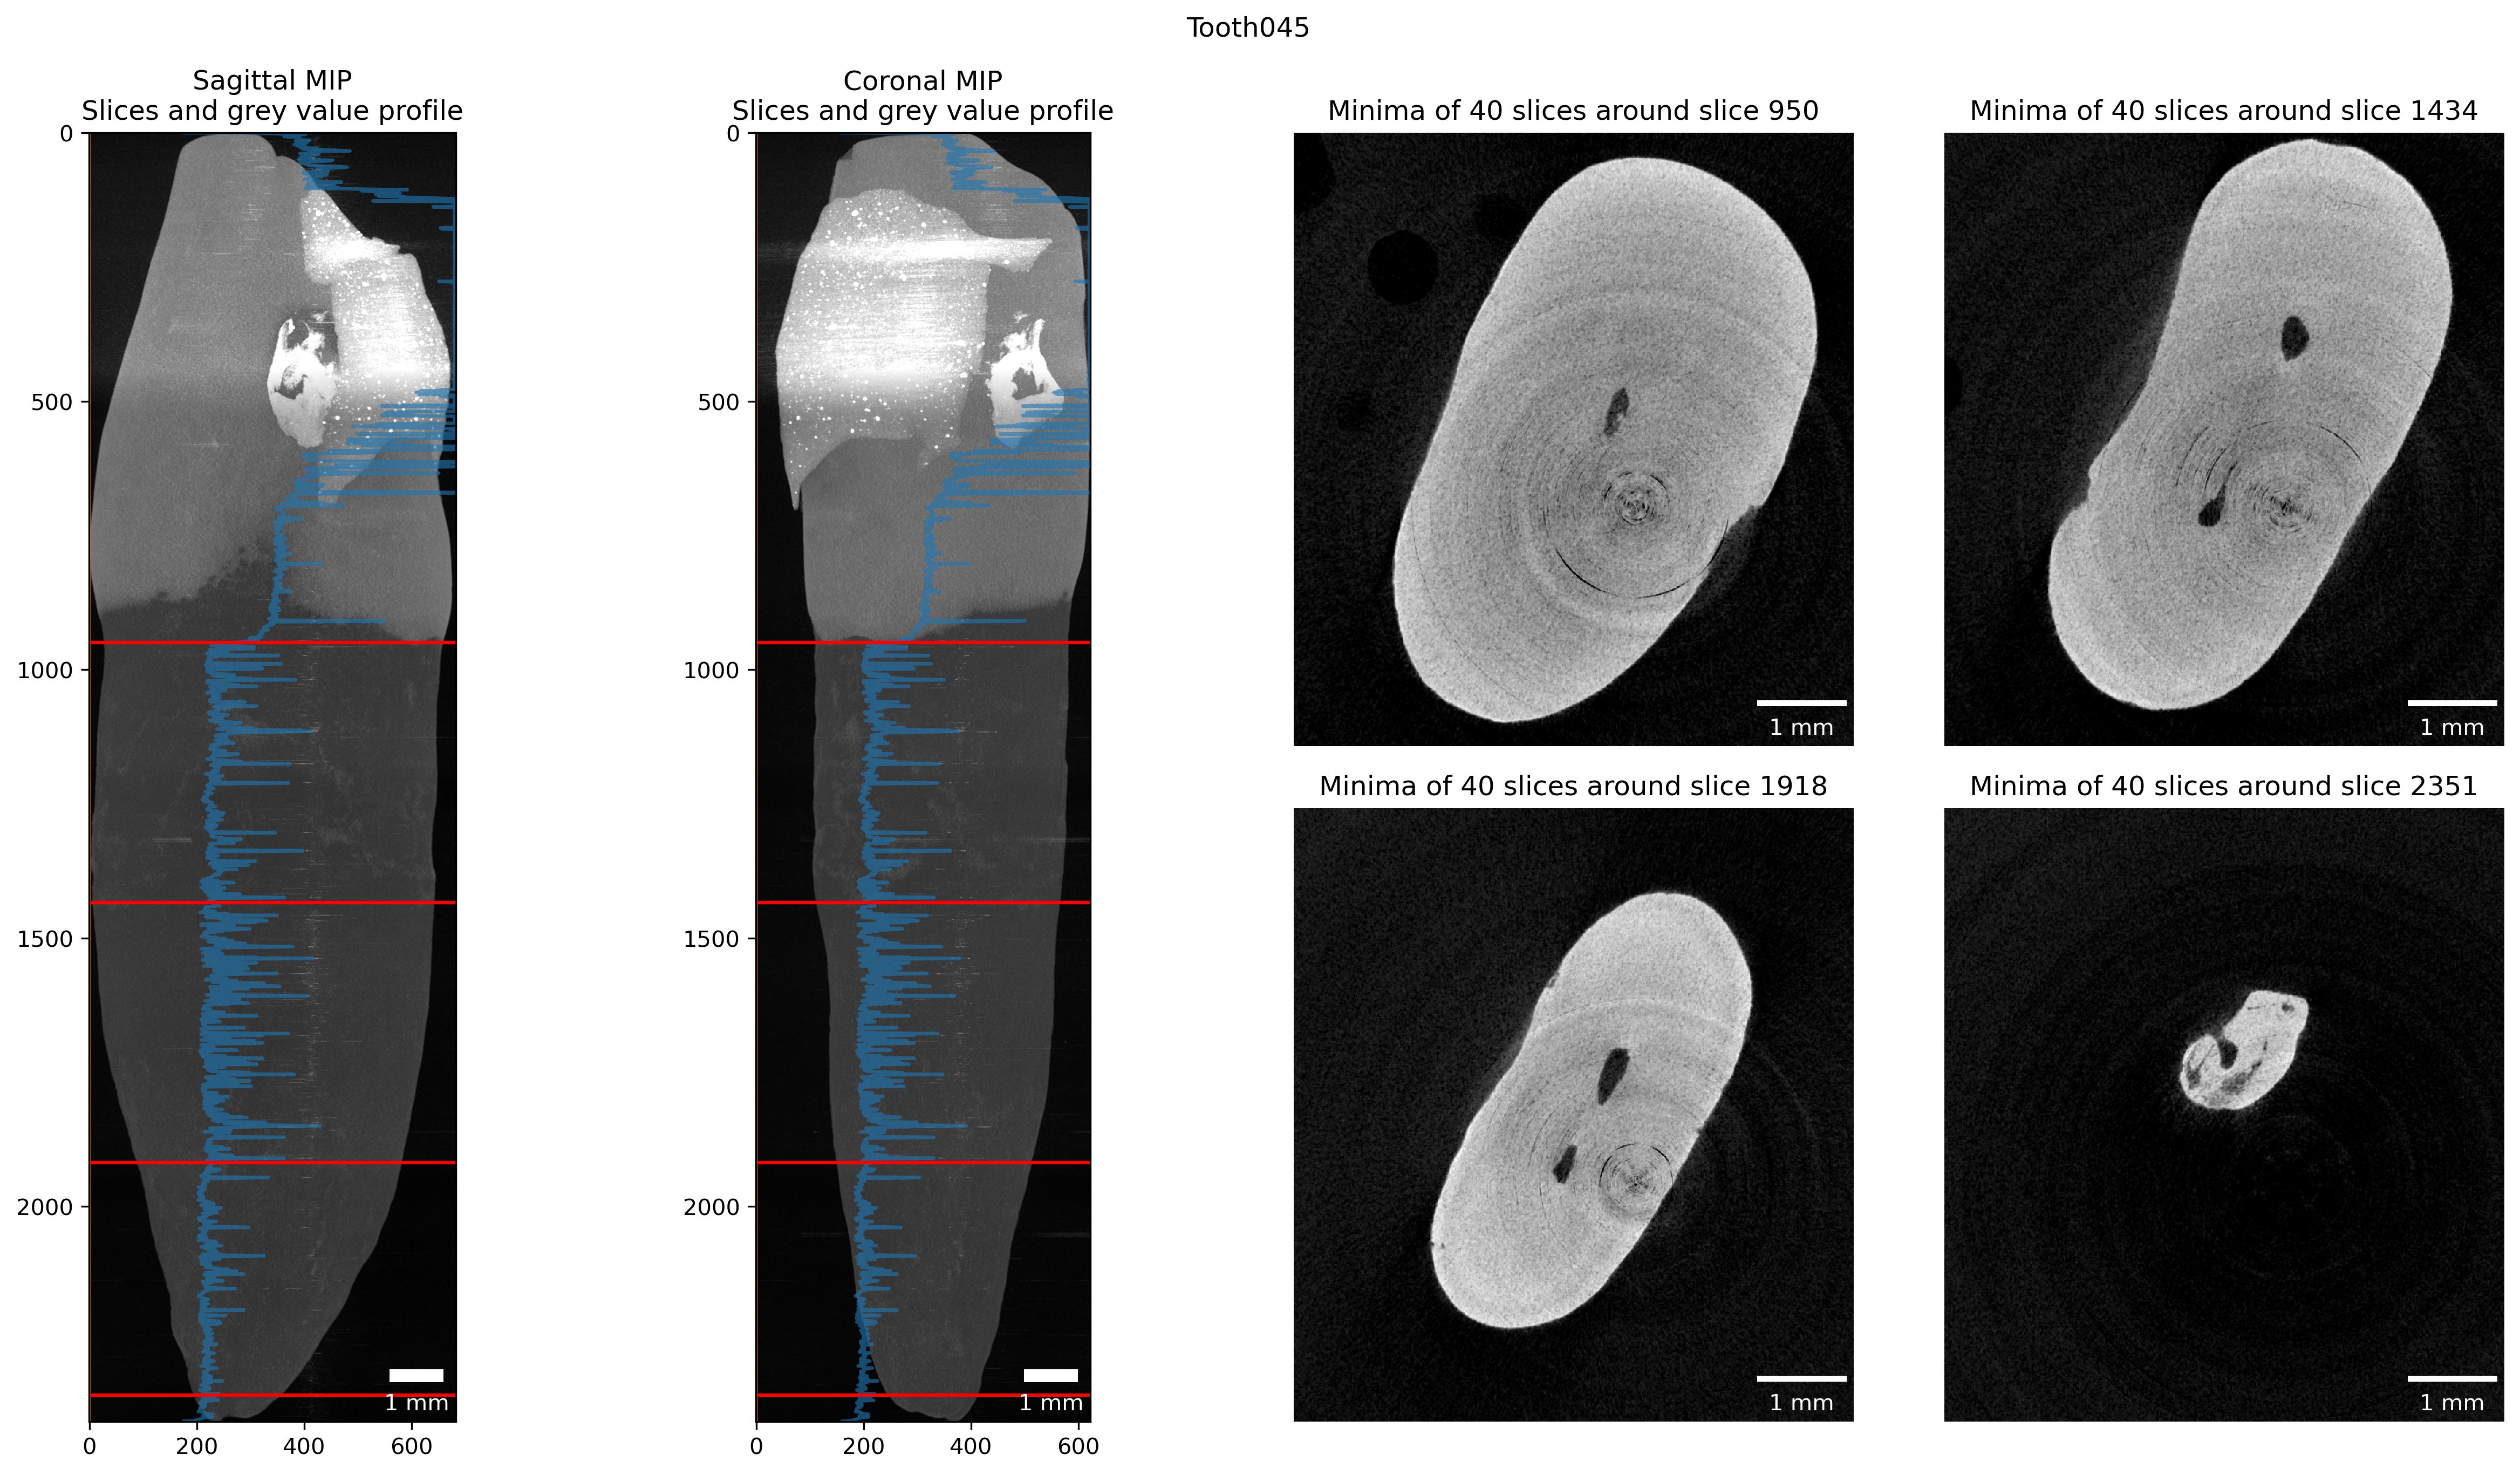
\includegraphics[height=\imheight]{{./images/tooth045/Tooth045.ExtractedSlices}}%
		}%
	\only<2|handout:2>{%
		\includegraphics[width=\linewidth]{{./images/tooth045/Tooth045.Briseno}}%
		}%
\end{frame}

\begin{frame}
	\frametitle{Extraction of root canal space}
	\begin{tikzpicture}[remember picture,overlay]%
	\node at (current page.center) [shift={(0,-25pt)}]{%
		\only<1|handout:0>{%
			\mode<beamer>{%
				\animategraphics[autoplay,loop,width=\paperwidth,every=\everyframe]{24}{./movies/tooth045/transparent-slices/image0}{000}{473}%
				}%
			\mode<handout>{%
				\includegraphics[width=\paperwidth]{./movies/tooth045/transparent-slices/image0000}%
				}%
			}%
		\only<2|handout:1>{%
			\mode<beamer>{%
				\animategraphics[autoplay,loop,width=\paperwidth,every=\everyframe]{24}{./movies/tooth045/transparent-slices-rcs/image0}{000}{457}%
				}%
			\mode<handout>{%
				\includegraphics[width=\paperwidth]{./movies/tooth045/transparent-slices-rcs/image0000}%
				}%
			}%
		\only<3|handout:0>{%
			\mode<beamer>{%
				\animategraphics[autoplay,loop,width=\paperwidth,every=\everyframe]{24}{./movies/tooth045/rcs/image0}{000}{413}%
				}%
			\mode<handout>{%
				\includegraphics[width=\paperwidth]{./movies/tooth045/rcs/image0000}%
				}%
			}%
		};%
	\end{tikzpicture}%
\end{frame}

\begin{frame}
	\frametitle{Results of root canal space extraction}%
		\includegraphics[height=\imheight]{./images/rcs/Tooth0452}%
		\includegraphics[height=\imheight]{./images/rcs/Tooth0278}%
		\includegraphics[height=\imheight]{./images/rcs/Tooth0353}%
		\includegraphics[height=\imheight]{./images/rcs/Tooth0419}%
		\includegraphics[height=\imheight]{./images/rcs/Tooth0642}%
		\includegraphics[height=\imheight]{./images/rcs/Tooth0752}%
		% Measuring the tooth length on Tooth093_rec_spr.bmp gives us 2092 pixels. We scanned at 10um.
		% "python ~/P/Dev/latex/draw_a_scalebar.py -i Tooth0931.png -l 2092 -p 10" gives us a scale bar
		\renewcommand{\imwidth}{0.358565737*\imheight}% 720/2008
		\pgfmathsetlength{\imagewidth}{\imwidth}%
		\pgfmathsetlength{\imagescale}{\imagewidth/720}%
		\def\x{72}% scalebar-x starting at golden ratio of image width of 720px = 445
		\def\y{1807}% scalebar-y at 90% of image height of 2008px = 1807
		\begin{tikzpicture}[x=\imagescale,y=-\imagescale]
				\node[anchor=north west, inner sep=0pt, outer sep=0pt] at (0,0) {\includegraphics[width=\imagewidth]{./images/rcs/Tooth0931}};
				% 1760.469px = 20.92mm -> 100px = 1188.319um -> 42.076px = 500um, 8.415px = 100um
				%\draw[|-|,blue,thick] (300,105) -- (327,1865) node [sloped,midway,above,fill=white,semitransparent,text opacity=1] {\SI{20.92}{\milli\meter} (1760px) TEMPORARY!};
				\draw[|-|,white,thick,shadowed] (\x,\y) -- (\x+420.76,\y) node [midway,above] {\shadowtext{\SI{5}{\milli\meter}}};
		\end{tikzpicture}%
\end{frame}

\begin{frame}
	\frametitle{Conclusion}
	\begin{itemize}
		\item Efficient use of time, \eg more teeth does not mean more (human) work
		\item Reproducible analysis with \emph{free and open-source} software, usable by \emph{anyone}
		\item Objective analysis, \eg no operator bias
	\end{itemize}
\end{frame}

\begin{frame}
	\frametitle{Thanks!}
	\begin{itemize}
		\item Thanks for listening to me!
		\item<2-> \href{https://twitter.com/jackiantonovich/status/1195699076056178691}{What questions do you have for me?}
	\end{itemize}
	\only<3|handout:0>{%
		\begin{tikzpicture}[remember picture,overlay]%
			\node at (current page.center){%
				\animategraphics[loop,autoplay,width=\paperwidth,every=\everyframe]{24}{./movies/mouse_skull/mouse_skull}{000}{236}%
				};%
		\end{tikzpicture}%
	}%
\end{frame}

\mode<beamer>{\begin{frame}[shrink=20]}
\mode<handout>{\begin{frame}[allowframebreaks]}
	\frametitle{References}
	\mode<beamer>{\renewcommand*{\bibfont}{\tiny}}
	\mode<handout>{\renewcommand*{\bibfont}{\scriptsize}}
	\setbeamertemplate{bibliography item}{\insertbiblabel}
	\printbibliography
\end{frame}

\begin{frame}
	\frametitle{\href{https://en.wikipedia.org/wiki/Colophon_(publishing)}{Colophon}}
	\begin{itemize}
		\item This \textsc{beamer} presentation was crafted in \LaTeX\xspace with the (slightly adapted) \href{http://intern.unibe.ch/dienstleistungen/corporate_design_und_vorlagen/praesentationen/index_ger.html}{template from \emph{Corporate Design und Vorlagen} of the University of Bern}.
		\begin{itemize}
			\item \href{https://github.com/habi/lecture.microtomography/}{Complete source code: git.io/fjpP7}
			\item The \LaTeX\xspace code is automatically compiled with a \href{https://github.com/actions}{GitHub action}\footnote{Details on how this works are specified in a \href{https://github.com/habi/latex-test/}{small test repository here: git.io/JeOOj}} to a \href{https://habi.github.io/Lecture.Microtomography/XRayMicroTomography.Handout.pdf}{(handout) PDF which you can access here: git.io/JeQxO}
		\end{itemize}
		\item Did you spot an error?
		\begin{itemize}
			\item \href{https://github.com/habi/lecture.microtomography/issues}{File an issue: git.io/fjpPb}
			\item \href{https://github.com/habi/lecture.microtomography/pulls}{Submit a pull request: git.io/fjpPN}
			\item \href{mailto:david.haberthuer@unibe.ch?subject=Error\%20in\%20the\%20(micro)-tomography\%20lecture\&body=https://xkcd.com/386/}{Send me an email: david.haberthuer@unibe.ch}
		\end{itemize}
	\end{itemize}
\end{frame}

\end{document}